\section{Results}
\label{sec:results}

% NOTE TO AUTHORS: every number in this section is a placeholder (\tbd). The tables and
% figures are laid out for the final results; fill them from results/*.json and
% results/p3-report.md once the corresponding step has run.

\Cref{tab:gosteps} records the outcome of the pre-registered go/no-go steps. The results below are reported in the order of the research questions.

\begin{table}[t]
\caption{Outcome of the pre-registered go/no-go steps (\cref{sec:eval-sim}).}
\label{tab:gosteps}
\small
\begin{tabular}{@{}llll@{}}
\toprule
Step & Criterion & Measured & Outcome \\
\midrule
G0 & (i) mean $|\hat\theta-\theta|\le0.05$ & \tbd & \tbd \\
   & (ii) hidden $F_1\ge0.6$; ambiguity $F_1\ge0.4$ & \tbd\,/\,\tbd & \tbd \\
   & (iii) regime criteria (four points, three types) & \tbd & \tbd \\
G1 & no collapse; R-SO typed hidden if observable & \tbd & \tbd \\
G2 & $\ge4$ acting models, $\ge2$ families & \tbd & \tbd \\
G3 & smoke checks; $\theta_m\ge0.5$ for every model & \tbd & \tbd \\
Gate & $\ge3$ wins of 4 on the development split & \tbd & \tbd \\
\bottomrule
\end{tabular}
\end{table}

%-------------------------------------------------------------------------------------------
\subsection{RQ1: Identifiability in practice}
\label{sec:results-rq1}

\Cref{tab:sim} reports accuracy recovery and simulated typed $F_1$ at the calibrated point and under the two misspecification arms. \Cref{fig:regime} shows the regime map, and \cref{fig:sim-n} shows how $F_1$ grows with the number of readings per model and cell.

\begin{table}[t]
\caption{Simulation at the calibrated point and under the misspecification arms. Typed $F_1$ (mean over replicates, with 95\% interval). Contradictions are symbolic and are not simulated.}
\label{tab:sim}
\small
\begin{tabular}{@{}l ccc ccc ccc@{}}
\toprule
 & \multicolumn{3}{c}{Calibrated} & \multicolumn{3}{c}{(A3) violated} & \multicolumn{3}{c}{(A5) violated} \\
\cmidrule(lr){2-4}\cmidrule(lr){5-7}\cmidrule(l){8-10}
Method & Hid. & Amb. & Weak & Hid. & Amb. & Weak & Hid. & Amb. & Weak \\
\midrule
\specdx (anchored cell model) & \tbd & \tbd & \tbd & \tbd & \tbd & \tbd & \tbd & \tbd & \tbd \\
Majority vote over models & \tbd & \tbd & \tbd & \tbd & \tbd & \tbd & \tbd & \tbd & \tbd \\
Deviates from anchor & \tbd & \tbd & \tbd & \tbd & \tbd & \tbd & \tbd & \tbd & \tbd \\
Joint-class latent model & \tbd & \tbd & \tbd & \tbd & \tbd & \tbd & \tbd & \tbd & \tbd \\
\midrule
\multicolumn{10}{@{}l}{Mean accuracy error $|\hat\theta_m-\theta_m|$ of \specdx: \tbd\ (calibrated), \tbd\ (A3), \tbd\ (A5); non-converged fits: \tbd} \\
\bottomrule
\end{tabular}
\end{table}

\begin{figure}[t]
\centering
\newcommand{\regimepanel}[3]{%
  \begin{scope}[shift={(#1)}]
    \node[font=\scriptsize\bfseries, anchor=south] at (1.25,1.65) {#2};
    \foreach \i in {0,...,4} {\foreach \j in {0,1,2} {
      \draw[gray!60, fill=white] (\i*0.5,\j*0.5) rectangle ++(0.5,0.5);
      \node[font=\tiny, gray] at (\i*0.5+0.25,\j*0.5+0.25) {--};
    }}
    \foreach \a [count=\i from 0] in {.6,.7,.8,.9,.95} {\node[font=\tiny, anchor=north] at (\i*0.5+0.25,0) {\a};}
    #3
  \end{scope}}
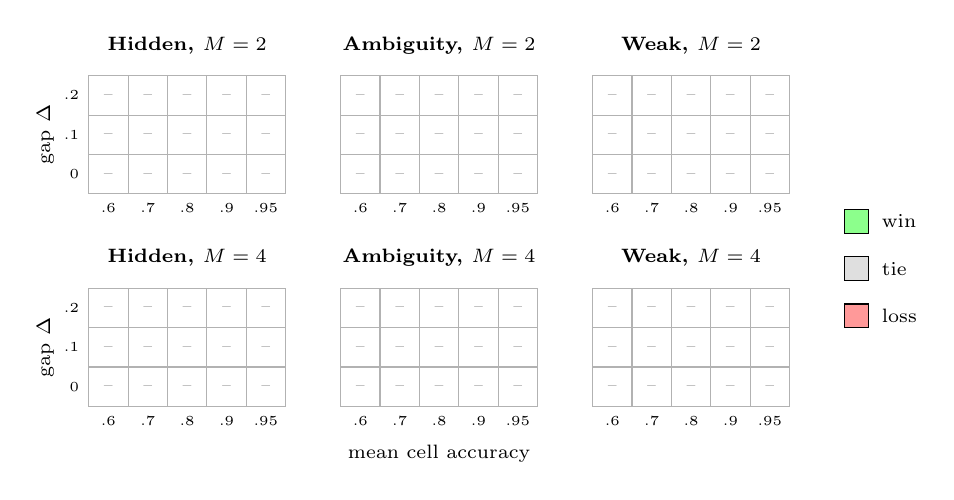
\begin{tikzpicture}
  \regimepanel{0,2.7}{Hidden, $M=2$}{\foreach \d [count=\j from 0] in {0,.1,.2} {\node[font=\tiny, anchor=east] at (0,\j*0.5+0.25) {\d};}\node[font=\scriptsize, rotate=90] at (-0.55,0.75) {gap $\Delta$};}
  \regimepanel{3.2,2.7}{Ambiguity, $M=2$}{}
  \regimepanel{6.4,2.7}{Weak, $M=2$}{}
  \regimepanel{0,0}{Hidden, $M=4$}{\foreach \d [count=\j from 0] in {0,.1,.2} {\node[font=\tiny, anchor=east] at (0,\j*0.5+0.25) {\d};}\node[font=\scriptsize, rotate=90] at (-0.55,0.75) {gap $\Delta$};}
  \regimepanel{3.2,0}{Ambiguity, $M=4$}{}
  \regimepanel{6.4,0}{Weak, $M=4$}{}
  \node[font=\scriptsize] at (4.45,-0.6) {mean cell accuracy};
  \begin{scope}[shift={(9.6,0.6)}, font=\scriptsize]
    \draw[fill=green!45] (0,1.6) rectangle ++(0.3,0.3); \node[anchor=west] at (0.35,1.75) {win};
    \draw[fill=gray!25]  (0,1.0) rectangle ++(0.3,0.3); \node[anchor=west] at (0.35,1.15) {tie};
    \draw[fill=red!40]   (0,0.4) rectangle ++(0.3,0.3); \node[anchor=west] at (0.35,0.55) {loss};
  \end{scope}
\end{tikzpicture}
\caption{Regime map: \specdx against the best simple baseline in each cell of the simulation grid (margin $0.05$; at least five replicates per cell). Cells will be coloured win, tie or loss. The boundaries predicted by \cref{thm:t2,thm:t2prime,thm:t4} are to be overlaid.}
\label{fig:regime}
\end{figure}

\begin{figure}[t]
\centering
\begin{tikzpicture}
\begin{groupplot}[
  group style={group size=3 by 1, horizontal sep=10mm, y descriptions at=edge left},
  width=0.36\textwidth, height=0.28\textwidth,
  xmin=0, xmax=40, ymin=0, ymax=1,
  xlabel={readings per model and cell $n$}, ylabel={typed $F_1$},
  xtick={0,10,20,30,40}, ytick={0,0.2,0.4,0.6,0.8,1},
  tick label style={font=\scriptsize}, label style={font=\scriptsize}, title style={font=\footnotesize},
  legend style={font=\scriptsize, draw=none, legend columns=4, at={(-0.75,-0.42)}, anchor=north}]
\nextgroupplot[title={Hidden requirement}]
\nextgroupplot[title={Ambiguity}]
\nextgroupplot[title={Weak check}]
  \addlegendimage{black, thick, mark=*}\addlegendentry{\specdx}
  \addlegendimage{blue, thick, dashed, mark=square*}\addlegendentry{majority vote}
  \addlegendimage{red, thick, dotted, mark=triangle*}\addlegendentry{deviates from anchor}
  \addlegendimage{gray, thick, dashdotted, mark=diamond*}\addlegendentry{joint-class model}
\end{groupplot}
\end{tikzpicture}
\caption{Simulated typed $F_1$ against the number of readings per model and cell, at the calibrated point. Data to be added.}
\label{fig:sim-n}
\end{figure}

\paragraph{Accuracy recovery.} [To be written: how closely $\hat\theta_m$ tracks the true accuracy, and whether the multi-start EM avoids the collapse of the earlier model.]

\paragraph{Typing.} [To be written: typed $F_1$ against the simple baselines at the calibrated point; the effect of the (A3) and (A5) arms.]

\paragraph{Calibration.} \Cref{fig:calibration} compares the posterior defect probabilities with the observed frequency of planted defects. [To be written.]

\begin{figure}[t]
\centering
\begin{tikzpicture}
\begin{groupplot}[
  group style={group size=3 by 1, horizontal sep=10mm, y descriptions at=edge left},
  width=0.36\textwidth, height=0.36\textwidth,
  xmin=0, xmax=1, ymin=0, ymax=1,
  xlabel={posterior probability}, ylabel={observed frequency},
  xtick={0,0.25,0.5,0.75,1}, ytick={0,0.25,0.5,0.75,1},
  tick label style={font=\scriptsize}, label style={font=\scriptsize}, title style={font=\footnotesize},
  legend style={font=\scriptsize, draw=none, legend columns=3, at={(-0.75,-0.38)}, anchor=north}]
\nextgroupplot[title={$\Prob(A_c\neq\{d_c\})$ (hidden)}]
  \addplot[gray, dashed, domain=0:1] {x};
\nextgroupplot[title={$\Prob(|A_c|=2)$ (ambiguity)}]
  \addplot[gray, dashed, domain=0:1] {x};
\nextgroupplot[title={MAP posterior (weak check)}]
  \addplot[gray, dashed, domain=0:1] {x};
  \addlegendimage{black, thick, mark=*}\addlegendentry{calibrated point}
  \addlegendimage{blue, thick, dashed, mark=square*}\addlegendentry{(A3) violated}
  \addlegendimage{red, thick, dotted, mark=triangle*}\addlegendentry{(A5) violated}
\end{groupplot}
\end{tikzpicture}
\caption{Calibration of the posterior defect probabilities in simulation (reliability diagrams, ten bins). The dashed diagonal is perfect calibration. Data to be added.}
\label{fig:calibration}
\end{figure}

\paragraph{Regimes.} [To be written: where \specdx wins, ties or loses; agreement of the empirical boundaries with \cref{thm:t2,thm:t2prime,thm:t4}.]

\rqanswer{1}{[To be completed once the results are final.]}

%-------------------------------------------------------------------------------------------
\subsection{RQ2: Effectiveness on seeded defects}
\label{sec:results-rq2}

\Cref{tab:main} gives typed $F_1$ per defect type, average precision and Detection@$k$ on the scorable mutants of the test split. Every method runs at its native protocol (Table A). \Cref{tab:paired} gives the paired comparisons, and \cref{fig:f1bars} shows typed $F_1$ by type. The corresponding tables for all mutants and for the development split are in the supplementary material.

\begin{table}[t]
\caption{Table A: effectiveness on scorable test mutants, every method at its native protocol. Typed $F_1$ per type; mean AP and Detection@$k$ over types the method reports; cost in model requests. ``\nr'' marks a type the method does not report. Scorable mutants per type: \tbd\,/\,\tbd\,/\,\tbd\,/\,\tbd.}
\label{tab:main}
\small
\setlength{\tabcolsep}{4.5pt}
\begin{tabular}{@{}l cccc c ccc r@{}}
\toprule
 & \multicolumn{4}{c}{Typed $F_1$} & & \multicolumn{3}{c}{Detection@$k$} & \\
\cmidrule(lr){2-5}\cmidrule(lr){7-9}
Method & Con. & Hid. & Amb. & Weak & AP & 1 & 3 & 5 & Requests \\
\midrule
\specdx & \tbd & \tbd & \tbd & \tbd & \tbd & \tbd & \tbd & \tbd & \tbd \\
\midrule
B1 BenchGuard & \tbd & \tbd & \tbd & \tbd & \tbd & \tbd & \tbd & \tbd & \tbd \\
B2 Who\&When & \nr & \tbd & \nr & \nr & \tbd & \tbd & \tbd & \tbd & \tbd \\
B3 IRT audit & \nr & \tbd & \nr & \nr & \tbd & \tbd & \tbd & \tbd & \tbd \\
B4 Semantic entropy & \nr & \nr & \tbd & \nr & \tbd & \tbd & \tbd & \tbd & \tbd \\
B5 MUS on $\Chk$ & \tbd & \nr & \nr & \nr & \tbd & \tbd & \tbd & \tbd & \tbd \\
TI GLAD & \nr & \tbd & \nr & \nr & \tbd & \tbd & \tbd & \tbd & \tbd \\
TI Dawid--Skene & \nr & \tbd & \nr & \nr & \tbd & \tbd & \tbd & \tbd & \tbd \\
JEST & \nr & \tbd & \nr & \nr & \tbd & \tbd & \tbd & \tbd & \tbd \\
\midrule
B2-naive & \nr & \tbd & \nr & \nr & \tbd & \tbd & \tbd & \tbd & \tbd \\
B3-2PL & \nr & \tbd & \nr & \nr & \tbd & \tbd & \tbd & \tbd & \tbd \\
\bottomrule
\end{tabular}
\end{table}

\begin{table}[t]
\caption{Paired comparison on typed detection (scorable test mutants): risk difference \specdx $-$ baseline with 95\% bootstrap interval, and exact McNemar $p$-value after Holm correction. Only types the baseline reports are compared.}
\label{tab:paired}
\small
\begin{tabular}{@{}l l c c@{}}
\toprule
Baseline & Type & Risk difference [95\% CI] & $p_{\text{Holm}}$ \\
\midrule
B1 BenchGuard & each of four & \tbd\ [\tbd, \tbd] & \tbd \\
B2 Who\&When & \Dhid & \tbd\ [\tbd, \tbd] & \tbd \\
B3 IRT audit & \Dhid & \tbd\ [\tbd, \tbd] & \tbd \\
B4 Semantic entropy & \Damb & \tbd\ [\tbd, \tbd] & \tbd \\
B5 MUS on $\Chk$ & \Dcon & \tbd\ [\tbd, \tbd] & \tbd \\
TI (best of GLAD, DS) & \Dhid & \tbd\ [\tbd, \tbd] & \tbd \\
JEST & \Dhid & \tbd\ [\tbd, \tbd] & \tbd \\
\bottomrule
\end{tabular}
\end{table}

\begin{figure}[t]
\centering
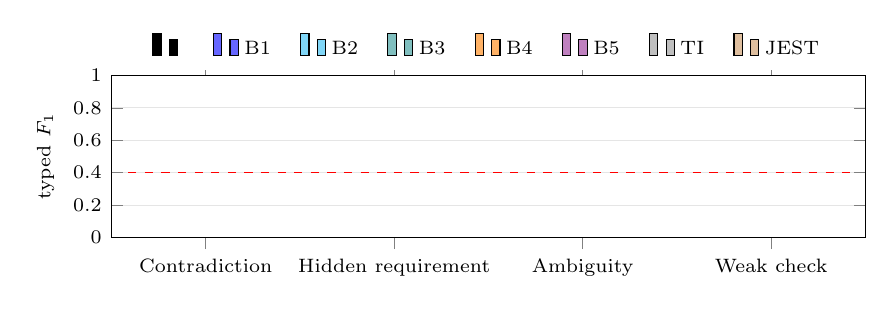
\begin{tikzpicture}
\begin{axis}[
  width=0.92\textwidth, height=0.3\textwidth,
  ybar, bar width=4pt, ymin=0, ymax=1, xmin=0.5, xmax=4.5,
  xtick={1,2,3,4}, xticklabels={Contradiction, Hidden requirement, Ambiguity, Weak check},
  ylabel={typed $F_1$}, ytick={0,0.2,0.4,0.6,0.8,1},
  tick label style={font=\scriptsize}, label style={font=\scriptsize},
  ymajorgrids, grid style={gray!20},
  legend style={font=\scriptsize, draw=none, legend columns=8, at={(0.5,1.03)}, anchor=south, /tikz/every even column/.append style={column sep=3mm}},
  extra y ticks={0.4}, extra y tick style={grid=major, major grid style={red, dashed}}, extra y tick labels={}]
  \addlegendimage{ybar, ybar legend, fill=black}\addlegendentry{\specdx}
  \addlegendimage{ybar, ybar legend, fill=blue!60}\addlegendentry{B1}
  \addlegendimage{ybar, ybar legend, fill=cyan!50}\addlegendentry{B2}
  \addlegendimage{ybar, ybar legend, fill=teal!50}\addlegendentry{B3}
  \addlegendimage{ybar, ybar legend, fill=orange!60}\addlegendentry{B4}
  \addlegendimage{ybar, ybar legend, fill=violet!50}\addlegendentry{B5}
  \addlegendimage{ybar, ybar legend, fill=gray!50}\addlegendentry{TI}
  \addlegendimage{ybar, ybar legend, fill=brown!50}\addlegendentry{JEST}
\end{axis}
\end{tikzpicture}
\caption{Typed $F_1$ by defect type on scorable test mutants, with 95\% bootstrap intervals. The dashed line marks the $0.4$ bar of the development gate for ambiguity and weak checks. Data to be added.}
\label{fig:f1bars}
\end{figure}

\paragraph{Contradictions.} [To be written.]

\paragraph{Hidden requirements.} [To be written.]

\paragraph{Ambiguities and localisation.} [To be written, including the share of ambiguities that ddmin localised and the size of the reported sentence sets.]

\paragraph{Weak checks.} [To be written.]

\paragraph{False positives on the base specification.} \Cref{fig:base-findings} shows the findings each method reports on the unmutated base specification. [To be written: the number of findings by type, and how many fall on the Unobservable list.]

\begin{figure}[t]
\centering
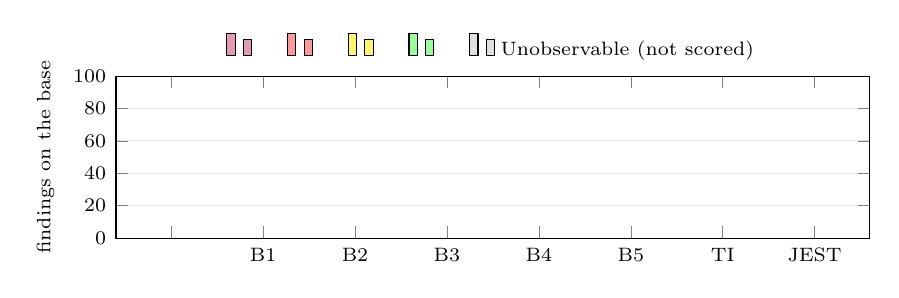
\begin{tikzpicture}
\begin{axis}[
  width=0.92\textwidth, height=0.3\textwidth,
  ybar stacked, bar width=10pt, ymin=0, ymax=100, xmin=0.4, xmax=8.6,
  xtick={1,...,8}, xticklabels={\specdx, B1, B2, B3, B4, B5, TI, JEST},
  ylabel={findings on the base}, tick label style={font=\scriptsize}, label style={font=\scriptsize},
  ymajorgrids, grid style={gray!20},
  legend style={font=\scriptsize, draw=none, legend columns=5, at={(0.5,1.03)}, anchor=south},
  /tikz/every even column/.append style={column sep=3mm}]
  \addlegendimage{ybar, ybar legend, fill=purple!40}\addlegendentry{\Dcon}
  \addlegendimage{ybar, ybar legend, fill=red!40}\addlegendentry{\Dhid}
  \addlegendimage{ybar, ybar legend, fill=yellow!60}\addlegendentry{\Damb}
  \addlegendimage{ybar, ybar legend, fill=green!40}\addlegendentry{\Dweak}
  \addlegendimage{ybar, ybar legend, fill=gray!25}\addlegendentry{Unobservable (not scored)}
\end{axis}
\end{tikzpicture}
\caption{Findings on the unmutated base specification, by type. Real defects among them are counted in \cref{sec:results-rq3}; the rest are candidate false positives. The y-axis range is a placeholder. Data to be added.}
\label{fig:base-findings}
\end{figure}

\rqanswer{2}{[To be completed once the results are final.]}

%-------------------------------------------------------------------------------------------
\subsection{RQ3: Real defects}
\label{sec:results-rq3}

\Cref{tab:real-results} reports, for each real defect, whether each method reports it with the right type and location, at what rank, and after how many population runs.

\begin{table}[t]
\caption{Real defects. \checkmark: reported with matching type and location; $\circ$: reported untyped or mislocated; $\times$: not reported; ``unobs.'': not observable by the population. Rank among the method's findings and population runs until first report (\specdx only).}
\label{tab:real-results}
\small
\begin{tabular}{@{}l ccc ccccccc@{}}
\toprule
 & \multicolumn{3}{c}{\specdx} & & & & & & & \\
\cmidrule(lr){2-4}
Defect & Found & Rank & Runs & B1 & B2 & B3 & B4 & B5 & TI & JEST \\
\midrule
R-SO (\Dhid) & \tbd & \tbd & \tbd & \tbd & \tbd & \tbd & \nr & \nr & \tbd & \tbd \\
R-12 (\Dcon) & \tbd & \tbd & \tbd & \tbd & \nr & \nr & \nr & \tbd & \nr & \nr \\
R-DE (\Dhid) & \tbd & \tbd & \tbd & \tbd & \tbd & \tbd & \nr & \nr & \tbd & \tbd \\
\bottomrule
\end{tabular}
\end{table}

\Cref{fig:rso} looks inside the anchored cell model at the R-SO cell: the share of readings that move away from the anchor for each model, and the posterior over the cell's candidate sets.

\begin{figure}[t]
\centering
\begin{tikzpicture}
\begin{groupplot}[
  group style={group size=2 by 1, horizontal sep=16mm},
  width=0.46\textwidth, height=0.32\textwidth,
  tick label style={font=\scriptsize}, label style={font=\scriptsize}, title style={font=\footnotesize}]
\nextgroupplot[title={(a) readings by model}, ybar stacked, bar width=12pt, ymin=0, ymax=1, xmin=0.4, xmax=4.6,
  xtick={1,...,4}, xticklabels={model 1, model 2, model 3, model 4}, ylabel={share of acted readings},
  xlabel={models ordered by $\hat\theta_m$},
  legend style={font=\scriptsize, draw=none, at={(0.5,-0.42)}, anchor=north, legend columns=3}]
  \addlegendimage{ybar, ybar legend, fill=orange!40}\addlegendentry{\vi{Chờ duyệt} ($d_c$)}
  \addlegendimage{ybar, ybar legend, fill=green!40}\addlegendentry{\vi{Đã duyệt}}
  \addlegendimage{ybar, ybar legend, fill=gray!30}\addlegendentry{other}
\nextgroupplot[title={(b) posterior over $A_c$}, ybar, bar width=12pt, ymin=0, ymax=1, xmin=0.4, xmax=5.6,
  xtick={1,...,5}, xticklabels={{$\{d_c\}$}, {\{\vi{Đã}\}}, {$\{d_c$, \vi{Đã}$\}$}, {$\emptyset$}, {other}},
  ylabel={posterior probability}, extra y ticks={0.5}, extra y tick style={grid=major, major grid style={red, dashed}}, extra y tick labels={}]
\end{groupplot}
\end{tikzpicture}
\caption{Inside the diagnosis of R-SO. (a)~For each model, the share of its acted readings of the cell \texttt{SO-0031}.status that equal the anchor, the alternative reading, or something else. (b)~The posterior over the cell's candidate sets; the dashed line marks $\tau_H$. Data to be added.}
\label{fig:rso}
\end{figure}

[To be written: discussion of each real defect, including the witness that \specdx reports and, for R-12, the synthesised scenario that exposed it. R-DOC is discussed qualitatively for B1.]

\rqanswer{3}{[To be completed once the results are final.]}

%-------------------------------------------------------------------------------------------
\subsection{RQ4: Cost-effectiveness}
\label{sec:results-rq4}

\Cref{fig:anytime} shows the detection rate of \specdx at its anytime checkpoints, together with the native cost of each baseline. \Cref{tab:equalcost} compares each LLM-based baseline with \specdx at equal cost (Table B).

\begin{figure}[t]
\centering
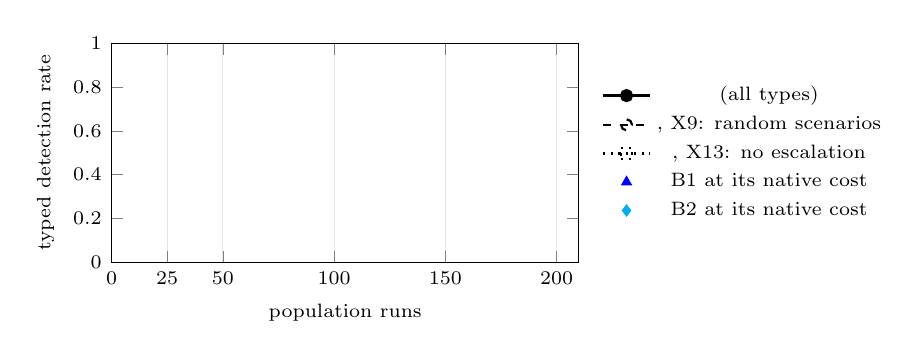
\begin{tikzpicture}
\begin{axis}[
  width=0.62\textwidth, height=0.36\textwidth,
  xmin=0, xmax=210, ymin=0, ymax=1,
  xtick={0,25,50,100,150,200}, ytick={0,0.2,0.4,0.6,0.8,1},
  xlabel={population runs}, ylabel={typed detection rate},
  tick label style={font=\scriptsize}, label style={font=\scriptsize},
  xmajorgrids, grid style={gray!20},
  legend style={font=\scriptsize, draw=none, at={(1.03,0.5)}, anchor=west}]
  \addlegendimage{black, thick, mark=*}\addlegendentry{\specdx (all types)}
  \addlegendimage{black, thick, dashed, mark=o}\addlegendentry{\specdx, X9: random scenarios}
  \addlegendimage{black, thick, dotted, mark=square}\addlegendentry{\specdx, X13: no escalation}
  \addlegendimage{only marks, mark=triangle*, blue}\addlegendentry{B1 at its native cost}
  \addlegendimage{only marks, mark=diamond*, cyan}\addlegendentry{B2 at its native cost}
\end{axis}
\end{tikzpicture}
\caption{Anytime behaviour: typed detection rate of \specdx at the checkpoints of 25, 50, 100, 150 and 200 population runs, with two ablations of the scenario policy. Ambiguities count as detected only at the final checkpoint, because localisation runs last. Data to be added.}
\label{fig:anytime}
\end{figure}

\begin{table}[t]
\caption{Table B: equal cost. Each LLM-based baseline at its native protocol, against \specdx at the checkpoint whose cost is closest to, and not above, the baseline's.}
\label{tab:equalcost}
\small
\begin{tabular}{@{}l r r cccc@{}}
\toprule
 & & \specdx & \multicolumn{4}{c}{Typed $F_1$ (baseline\,/\,\specdx)} \\
\cmidrule(l){4-7}
Baseline & Requests & checkpoint & Con. & Hid. & Amb. & Weak \\
\midrule
B1 BenchGuard & \tbd & \tbd & \tbd\,/\,\tbd & \tbd\,/\,\tbd & \tbd\,/\,\tbd & \tbd\,/\,\tbd \\
B2 Who\&When & \tbd & \tbd & \nr\,/\,\tbd & \tbd\,/\,\tbd & \nr\,/\,\tbd & \nr\,/\,\tbd \\
\bottomrule
\end{tabular}
\end{table}

\Cref{fig:cost} breaks the cost of each method down by what the requests were spent on.

\begin{figure}[t]
\centering
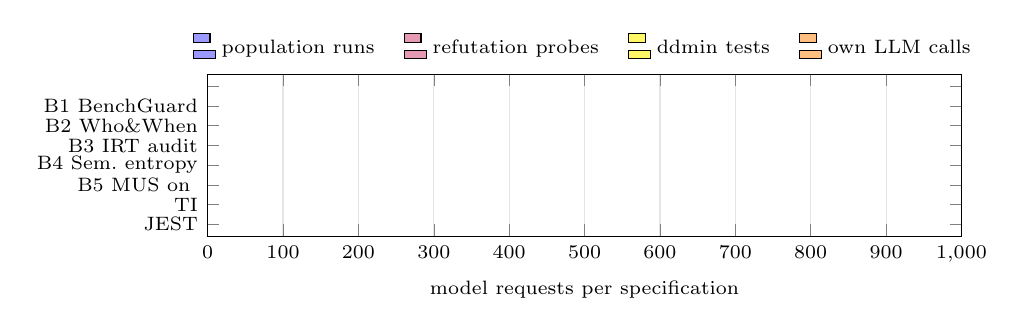
\begin{tikzpicture}
\begin{axis}[
  width=0.92\textwidth, height=0.3\textwidth,
  xbar stacked, bar width=8pt, xmin=0, xmax=1000, ymin=0.4, ymax=8.6,
  ytick={1,...,8}, yticklabels={\specdx, B1 BenchGuard, B2 Who\&When, B3 IRT audit, B4 Sem.\ entropy, B5 MUS on $\Chk$, TI, JEST},
  y dir=reverse, xlabel={model requests per specification},
  tick label style={font=\scriptsize}, label style={font=\scriptsize}, xmajorgrids, grid style={gray!20},
  legend style={font=\scriptsize, draw=none, legend columns=5, at={(0.5,1.03)}, anchor=south},
  /tikz/every even column/.append style={column sep=3mm}]
  \addplot[draw=none, forget plot] coordinates {(0,0.4) (0,8.6)};
  \addlegendimage{xbar, xbar legend, fill=blue!40}\addlegendentry{population runs}
  \addlegendimage{xbar, xbar legend, fill=purple!40}\addlegendentry{refutation probes}
  \addlegendimage{xbar, xbar legend, fill=yellow!60}\addlegendentry{ddmin tests}
  \addlegendimage{xbar, xbar legend, fill=orange!50}\addlegendentry{own LLM calls}
\end{axis}
\end{tikzpicture}
\caption{Cost per specification in model requests, by component. Baselines that consume \specdx's runs are charged those runs plus their own calls. The x-axis range is a placeholder. Data to be added.}
\label{fig:cost}
\end{figure}

[To be written: runs to first detection per type; the share of scenarios escalated; the cost of refutation and localisation relative to population runs; wall-clock time on the 48\,GB GPU.]

\rqanswer{4}{[To be completed once the results are final.]}

%-------------------------------------------------------------------------------------------
\subsection{RQ5: Ablation}
\label{sec:results-rq5}

\Cref{tab:ablation} reports the change in typed $F_1$ when one component is removed or replaced.

\begin{table}[t]
\caption{Ablation on the scorable mutants: change in typed $F_1$ relative to full \specdx (negative means the component helps).}
\label{tab:ablation}
\small
\begin{tabular}{@{}llcccc@{}}
\toprule
Id & Variant & Con. & Hid. & Amb. & Weak \\
\midrule
--  & Full \specdx (typed $F_1$) & \tbd & \tbd & \tbd & \tbd \\
\midrule
X1 & No anchor: latent truth without $d_c$ in the prior & \tbd & \tbd & \tbd & \tbd \\
X2 & Joint class over a whole step instead of cells & \tbd & \tbd & \tbd & \tbd \\
X3 & Free per-cell $\varepsilon_c$ instead of the flat pool & \tbd & \tbd & \tbd & \tbd \\
X4 & Per-cell instead of grouped difficulty & \tbd & \tbd & \tbd & \tbd \\
X5 & Single-truth Dawid--Skene instead of set-valued $A_c$ & \tbd & \tbd & \tbd & \tbd \\
X6 & No stage 1 (no observability gating) & \tbd & \tbd & \tbd & \tbd \\
X7 & Single-clause tests only (no hitting-set duality) & \tbd & \tbd & \tbd & \tbd \\
X8 & No refutation & \tbd & \tbd & \tbd & \tbd \\
X9 & Random scenarios instead of Thompson sampling & \tbd & \tbd & \tbd & \tbd \\
X10 & No T-boundary scenarios & \tbd & \tbd & \tbd & \tbd \\
X11 & Lexical-overlap localisation instead of ddmin & \tbd & \tbd & \tbd & \tbd \\
X12 & Two models instead of four & \tbd & \tbd & \tbd & \tbd \\
X13 & No escalation: always run the full population & \tbd & \tbd & \tbd & \tbd \\
\bottomrule
\end{tabular}
\end{table}

[To be written.]

\rqanswer{5}{[To be completed once the results are final.]}
